\documentclass[a4paper,dvipsnames]{article}

\input ../../header

\newcommand{\un}{\left(u_n\right)_{n\in\mathbb{N}}}
\newcommand{\uns}{\left(u_n\right)_{n\in\mathbb{N}^\ast}}
\newcommand{\vn}{\left(v_n\right)_{n\in\mathbb{N}}}
\newcommand{\vns}{\left(v_n\right)_{n\in\mathbb{N}^\ast}}
\newcommand{\wn}{\left(w_n\right)_{n\in\mathbb{N}}}
\newcommand{\wns}{\left(w_n\right)_{n\in\mathbb{N}^\ast}}
\newcommand{\tn}{\left(t_n\right)_{n\in\mathbb{N}}}
\newcommand{\tns}{\left(t_n\right)_{n\in\mathbb{N}^\ast}}
\newcommand{\qn}{\left(q_n\right)_{n\in\mathbb{N}}}
\newcommand{\qns}{\left(q_n\right)_{n\in\mathbb{N}^\ast}}
\newcommand{\N}{\mathbb{N}}

\title{Projet 2 -- Le parachute de Perseverance}

\author{}
\date{}

\begin{document}

\renewcommand{\contentsname}{}

\pagestyle{fancy}

\begin{tcolorbox}[colframe=blue!75, colback=blue!45, valign=center, height=1.5cm, top=5mm]
  \maketitle
\end{tcolorbox}

\tableofcontents

\vspace{1cm}

\thispagestyle{fancy}

\section{Introduction}

Le jeudi 18 février, le rover Perseverance de la NASA a atterri avec succès sur Mars. La \href{https://peertube-lyclpg.ddns.net:9443/videos/watch/6db70ede-ff84-432e-8542-e6f335db75a1}{vidéo} a été diffusée sur Internet. Alors que le parachute se déployait, les internautes ont repéré un étrange motif sur le parachute.

\medskip

Sur le très populaire forum Reddit, certains se sont demandés si cet étrange motif ne cachait pas un code. Il aura fallu moins de six heures aux internautes pour trouver le message caché dans ce parachute. 

\section{Le codage du parachute}

En observant avec attention, on se rend compte que le parachute comprend quatre cercles concentriques. Chacun de ces cercles est découpé en 80 sections, et ces sections peuvent être blanches ou rouges. Voici un schéma du parachute :

\begin{center}
  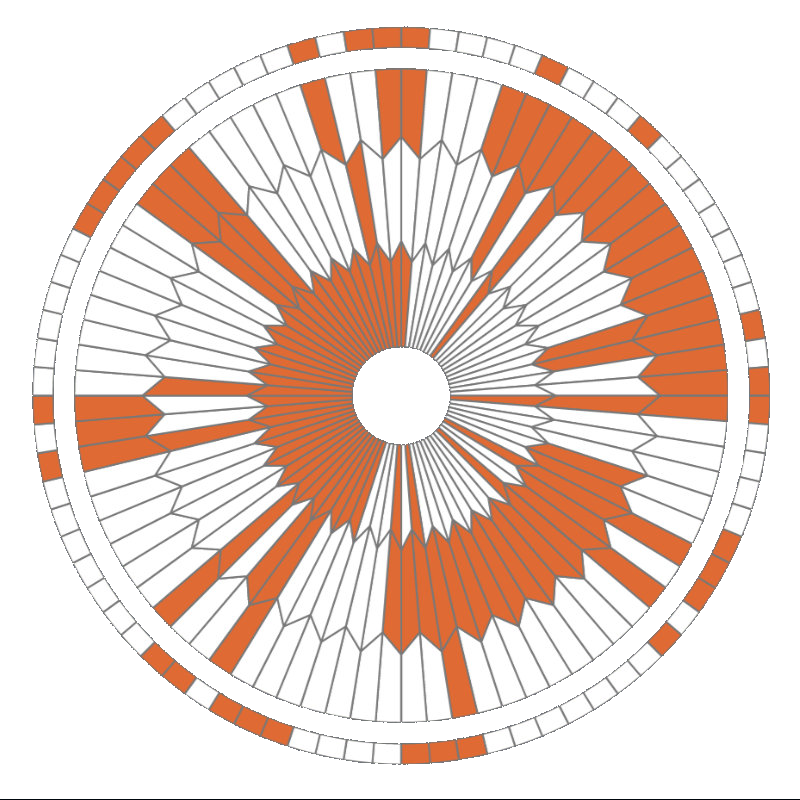
\includegraphics[width=10cm]{img/motif.png}
\end{center}

\subsection{La répartition des couleurs}

 En examinant de plus prêt le motif, les internautes sont parvenus à déchiffrer le message en cherchant avec des méthodes usuelles de cryptanalyse. Les trois anneaux centraux du parachute comprennent une zone rouge continue. Cette zone rouge sert à indiquer la fin du message.

\medskip

Les anneaux comprennent 80 éléments. On peut imaginer que ces 80 éléments indiquent 10 octets. Malheureusement, on ne parvient pas à déchiffrer le message caché de cette façon.

\medskip

Par contre, on peut faire 8 groupes de 10 bits commençant chacun par trois zéros (trois traits blancs). Le \og{}grand\fg{} groupe rouge continu commence lui aussi par 3 traits blancs. C'est ainsi que le codage a été trouvé. En appliquant ce principe, on regroupe les traits de la façon suivante dans l'anneau le plus interne :

\begin{center}
  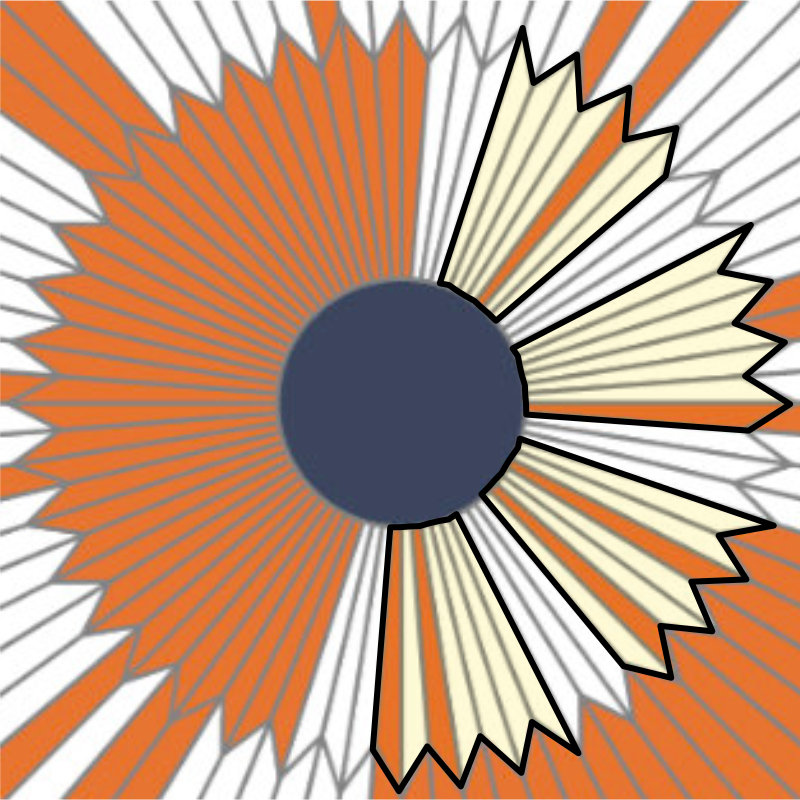
\includegraphics[width=10cm]{img/motif-colorie.png}
\end{center}

\subsection{Encodage}

\subsubsection{Anneau central}

 Cette répartition des couleurs correspond à un encodage en binaire. En considérant que le blanc signifie 0 et que le rouge signifie 1, on a donc :

 \begin{itemize}
   \item 000 0100 pour le premier groupe;
   \item 000 0001 pour le second groupe;
   \item 001 0010 pour le troisième groupe;
   \item 000 0101 pour le quatrième groupe.
 \end{itemize}
    
 Le premier groupe correspond en binaire au nombre 4. La quatrième lettre de l'alphabet est le D, et c'est aussi la première lettre du message martien. L'étrange message du parachute est donc chiffré en utilisant le code secret des enfants : A \og{}vaut\fg{} 1, B \og{}vaut\fg{} 2, C \og{}vaut\fg{} 3, etc.

\medskip

\begin{exercice}{}{}
  Indiquer à quel nombre correspondent les groupes suivants. En déduire la lettre qu'ils codent.
\end{exercice}

\subsubsection{Les deuxième et troisième anneau}

Le message contient trois mots (un par anneau intérieur). Les deuxième et troisième anneaux fonctionnent sur le même principe. Il suffit donc de faire des blocs de 10 bits et de déterminer à quel(le) nombre/lettre ils correspondent. 

\medskip

\begin{exercice}{}{}
 \begin{enumerate}
   \item Regrouper de la même façon les éléments du deuxième et du troisième anneau pour trouver le deuxième et le troisième mot du message. 
   \item L'ensemble des trois mots constitue la devise d'une célèbre institution. Laquelle ?
 \end{enumerate} 
\end{exercice}

\subsubsection{Le dernier anneau}

Le dernier anneau a laissé les internautes perplexes un peu plus longtemps. Et pour cause ! Les trois premiers anneaux contenaient des lettres, représentés par des nombres entre 1 et 26. Sur le quatrième et dernier anneau, on commence par un nombre qui vraisemblablement ne correspond pas à une lettre : 34 !

\begin{center}
  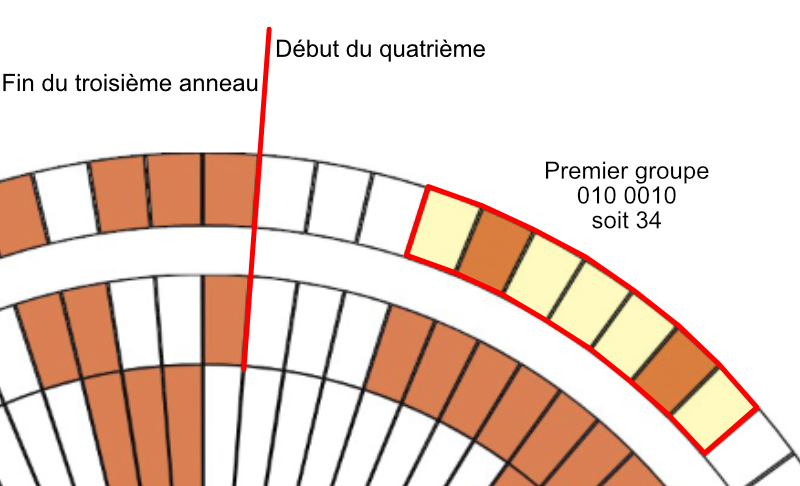
\includegraphics[width=10cm]{img/cercle-externe.png}
\end{center}

En fait, le 4ème cercle indique des coordonnées GPS. Il y a d'abord trois groupes de chiffres puis une lettre (S ou N) qui indique la latitude puis trois groupes de chiffres et une lettre (E pour est ou W pour ouest en anglais) qui indiquent la longitude.

\medskip

\begin{exercice}{}{}
  \begin{enumerate}
    \item Préciser les 8 groupes de bits.
    \item Traduire les trois premiers en chiffres et le quatrième en lettre.
    \item Faire de même avec les quatre autres groupes.
    \item À quel endroit correspondent ces coordonnées GPS ?
  \end{enumerate}
\end{exercice}

\pagebreak

\section{Un autre parachute}

On peut très bien coder d'autres messages sur le même principe. Voici une proposition qui contient un autre message :

\begin{center}
  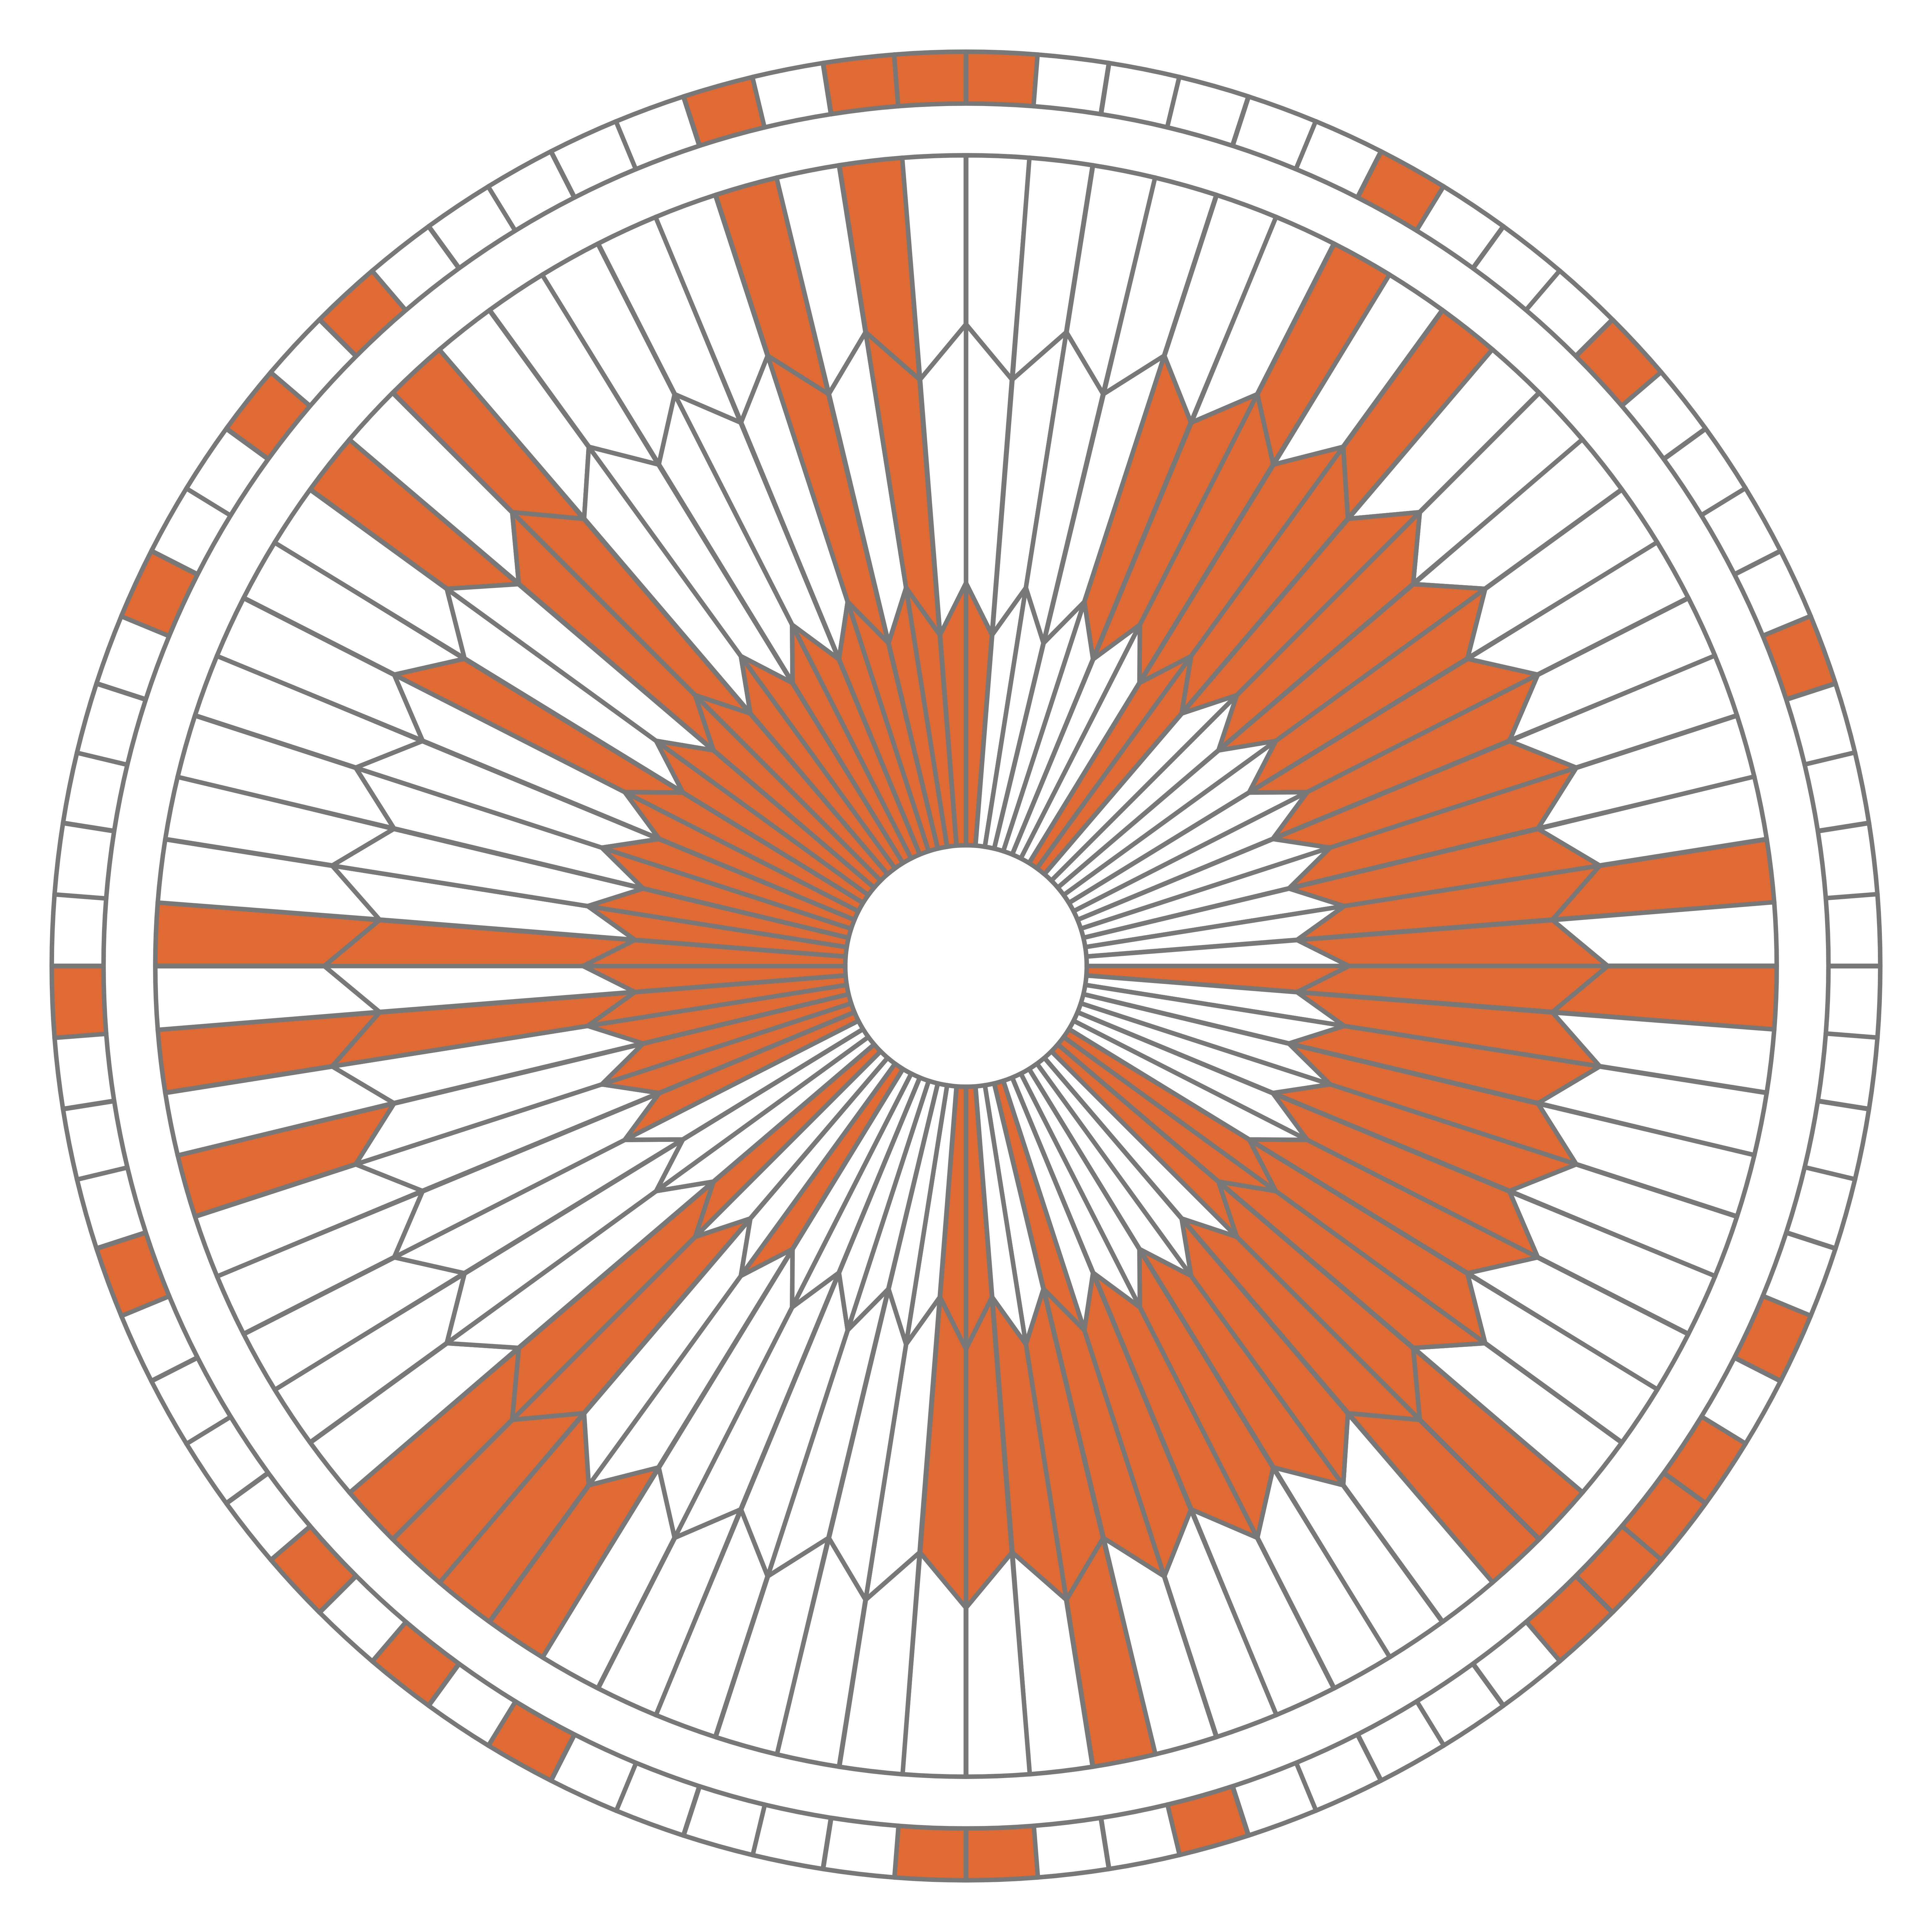
\includegraphics[width=10cm]{img/parachute-perso.png}
\end{center}

\begin{exercice}{}{}
  Traduire ce message et indiquer à quel batîment correspondent les coordonnées du dernier cercle.

  \tcblower

  \textit{Remarque : les entiers supérieurs à $127$ ont été représentés \og{}modulo $128$\fg{} (par exemple, $140$ aurait été représenté par $12$.}
\end{exercice}

\medskip

\begin{remarque}{}{}
  Vous pouvez générer votre propre parachute sur cette \href{https://sjwarner.github.io/perseverance-parachute-generator/}{page}.
\end{remarque}

\end{document}
